\documentclass[11pt]{article}

\usepackage[scale=0.75,a4paper]{geometry}
\usepackage[utf8]{inputenc}
\usepackage[british]{babel}
\usepackage{csquotes}
\usepackage{graphicx}
\usepackage{subcaption}
\usepackage{float}
\usepackage{amsmath}
% \usepackage{amssymb}
\usepackage[separate-uncertainty=true]{siunitx}
\usepackage{minted}
\usepackage{titling}
% \usepackage{lipsum}
\usepackage[
    backend=biber,
    style=numeric
]{biblatex}

\addbibresource{references.bib}

% ====== table cosmetics ======
% \renewcommand{\arraystretch}{1.3}
% \setlength{\tabcolsep}{18pt}

% ====== shortcuts ======
\newcommand{\R}[1]{\mathrm{#1}}
\newcommand{\CC}{{C\nolinebreak[4]\hspace{-.05em}\raisebox{.3ex}{\scriptsize\bf ++}}}

% ====== style the title ======
\setlength{\droptitle}{-25pt}
\pretitle{\begin{center} \LARGE}
\posttitle{\end{center}}
\preauthor{}
\postauthor{}
\predate{\begin{center} \large }
\postdate{\end{center}}



\begin{document}
\title{Optics with Imperfect Mirrors\\Part II Computational Project}
\author{}
\date{\today}
\maketitle

\abstract{
    Write fancy abstract here TODO.
}

\noindent\rule{0.85\textwidth}{0.4pt}


\section{Introduction}~\label{sec:intro}
Modern telescopes use very finely polished curved mirrors to create sharp images. However, errors are an inherent property of any physical system and any manufacturing process. Thus, regardless of the way mirrors are manufactured (e.g.\ spin-casting or polishing), there are still imperfections in their shape.

The aim of this paper is a computational investigation of the effects of imperfections in the shape of a telescope mirror on the image. Several relationships are studied, as suggested in the projects manual~\cite{manual}:
\begin{itemize}
    \item the effects of Gaussian illumination, where the amplitude of radiation on the mirror
    \begin{equation*}
        \left| A(r) \right| \propto \exp \left( -{r^2}/{2 \sigma_T^2} \right)
    \end{equation*}
    on the size and central intensity of the image.
    \item the effect of a central hole in the mirror, due to the secondary mirror.
    \item the effects of random and correlated phase errors, due to physical dents in the surface of the mirror. The dents cause phase errors due to the change in path length with respect to the smooth shape.
\end{itemize}

A more detailed analysis of the theory and techniques used is given in Section~\ref{sec:analysis}. Implementation details are discussed in Section~\ref{sec:impl}, and results are presented and discussed in Section~\ref{sec:res}.


\section{Analysis}~\label{sec:analysis}
In the analysis of this problem, we treat the far-field diffraction pattern of the mirror under uniform or Gaussian illumination. In the far field regime, the diffraction pattern of an aperture is given by the Fourier Transform of the aperture function \( A(x,y) \)~\cite[Chapter 10.2]{hecht}. This is a reasonable approximation as long as:
\begin{equation}\label{eqn:fraunhofer}
    \frac{R^2}{\lambda D} \ll 1,
\end{equation}
known as the Fraunhofer limit, where $R$ is the maximum extent of the aperture, $\lambda$ is the wavelength of radiation and $D$ is the distance from the aperture to the screen onto which the image is projected. In this problem we use:
\begin{align*}
    \lambda &= \SI{1}{mm} \\
    R &= \SI{6}{m},
\end{align*}
which would require a distance on the order of \SI{1}{km} for the far-field limit to hold. 

However, we can work in angular coordinates, with the image space spanned by:
\begin{align*}
    p &= k \sin{\theta} \approx \frac{k x'}{D} \\
    q &= k \sin{\chi} \approx \frac{k y'}{D},
\end{align*}
where $x'$ and $y'$ are distances that would span a physical image space, and $k$ is the wavenumber. We thus eliminate the dependence on $D$. In these coordinates, the image is given by:
\begin{equation}\label{eqn:diff}
    \psi(p, q) \propto \iint A(x, y) \exp \left( ipx + iqy \right) dx dy,
\end{equation}
which is just a Fourier transform of $A$. Seemingly we've also eliminated the dependence on $\lambda$, but that will be needed again in the analysis of dented mirrors (Section~\ref{sec:analysis:bent}).

\subsection{Discrete Fourier Transforms}\label{sec:analysis:dft}
The fact that the image is a Fourier transform of the aperture function is very useful. The Fast Fourier Transform algorithm can compute discrete Fourier transforms of multi-dimensional data efficiently, and there exist library implementations of it for virtually any language. Here, the \CC{} \texttt{FFTW 3} library~\cite{fftw} was chosen, as suggested in the projects manual~\cite{manual}. It is a well-established and well-tested library with very good computational efficiency.

Minor adaptations are required to use the DFT algorithms in the library. The 1D discrete Fourier transform is defined as~\cite[Chapter 12.1]{NumRecipes}:
\begin{equation}
    H_k \propto \sum_{n=0}^{N-1} h_n\ \exp{\left( 2\pi{}i \frac{kn}{N} \right)},
\end{equation}
with the corresponding frequency values:
\begin{equation}\label{eqn:fk}
    f_k = \frac{k}{N \Delta},\quad k = 0..N-1,
\end{equation}
where $\Delta$ is the sampling interval of the original signal. Comparing to a 1D discrete form of the diffraction integral (Equation~\ref{eqn:diff}): 
\begin{equation}
    \psi_k \propto \sum_{n=0}^{N-1} A_n \exp{\left( i p_k x_n \right)},\quad \R{where} \quad x_n = n \Delta
\end{equation}
we see that we need to rescale:
\begin{equation}
    p_k = 2\pi f_k
\end{equation}

\subsection{Testing}\label{sec:analysis:test}
To determine whether the algorithm is outputting something sensible, we need to test it on a range of known results. Diffraction patterns for several kinds of apertures are easy to compute analytically, and thus can be used for testing the program.

\paragraph{Rectangular aperture} A rectangular aperture of size $-a < x < a$, $-b < y < b$ has diffraction pattern:
\begin{equation}
    \psi(p, q) \propto \frac{\sin{\left( pa \right)}}{pa} \frac{\sin{\left( qb \right)}}{qb},
\end{equation}
thus it's expected to have the first zeros at:
\begin{equation}\label{eqn:test_rect}
    p = \pm \frac{\pi}{a}\quad \R{and} \quad q = \pm \frac{\pi}{b}.
\end{equation}

\paragraph{Circular aperture} A circular aperture of radius $R$ has a diffraction pattern called an Airy disc, with angular radius:
\begin{equation}\label{eqn:test_circ}
    \sin{\theta} \approx 1.22 \frac{\lambda}{2R} \quad \Rightarrow \quad p = 1.22 \frac{\pi}{R}.
\end{equation}

Both of these zero-intensity points should appear in the diffraction patterns, and the scaling with the inverse of the aperture size should be observable.

\subsection{Bent mirrors}\label{sec:analysis:bent}

\section{Implementation}\label{sec:impl}
The implementation consists of several different parts, discussed in the subsections that follow. The overall logic flow of the program is:
The executable is invoked with one argument, pointing to a configuration file. The instructions therein are read and executed in order, thus computing diffraction patterns for the described apertures. The results are printed to disk, and figures can then be produced by invoking the respective Python scripts for each problem.

\CC{} source files are in \texttt{src/cpp}, and plotting scripts in \texttt{src/scripts}. Data is written by convention to the \texttt{data} directory, and figures to \texttt{fig}.

\subsection{Describing Apertures and Images}
In the \texttt{FFTW} library two-dimensional $N_x$ by $N_y$ arrays are represented as one-dimensional $N_x \times N_y$ arrays of complex numbers (of the inbuilt \texttt{complex} type)~\cite[Section 3.2]{fftw}.

Because working directly with a 1D representation of 2D data can be clunky, I decided to wrap this functionality in a class called \texttt{Array2d}, declared in \texttt{array2d.h} and implemented in \texttt{array2d.cpp}. The class stores the data internally in the 1D array representation, but has a more user-friendly interface. For example, it defines the \texttt{[i][j]} and \texttt{(i, j)} operators for easy access to the element in the $i^{th}$ row and $j^{th}$ column.

\paragraph{FFTW compatibility} The method \texttt{ptr()} returns a pointer to the beginning of the array, cast to \texttt{fftw\_complex} type. This pointer can be passed to functions in the \texttt{FFTW} library~\cite[Section 4]{fftw}.

\paragraph{Memory allocation} One special feature of this class that breaks with convention is that there is no explicitly defined copy constructor. The compiler generated one only performs a shallow copy, copying the pointer to the data array, but not the data itself. Only the explicitly defined constructor \mintinline{C++}{Array2d::Array2d(int nx, int ny)} uses \texttt{fftw\_alloc\_complex} to allocate new memory for the array. This means that the user of the class has finer control over where memory is allocated, which is important in the case of large arrays. For example, using IEEE double-precision floating point, which occupies 64 bits of memory, a $2^{13} \times 2^{13}$ array of complex numbers occupies around \SI{1}{GB} of memory.

For better understanding of when new memory is allocated, compile the code with the variable \texttt{DEBUG\_OUT} set to \texttt{true} in \texttt{array2d.cpp}. Then the calls to the memory-allocating constructor of \texttt{Array2d} will be logged to standard output.

\paragraph{Aperture generators} These are a type of function that initialise an \texttt{Array2d} with a particular kind of aperture with given parameters. For example, there is a generator for circular apertures, one for circular Gaussian-illuminated, one for circular with random errors, etc.

\subsection{Configuration Files}
Configuration files are stored by convention in the \texttt{config} directory, and are a series of \texttt{key = value} lines. They contain:
\begin{itemize}
    \item \texttt{nx} and \texttt{ny}. These are the size of the problem, i.e.\ the numbers of rows and columns that the mirror shape is split into.
    \item \texttt{tasks}, what actions to perform on each of the shapes
    \item \texttt{n\_shapes}, the number of shapes
    \item for each shape, it's properties: \texttt{type}, \texttt{lx} and \texttt{ly}, the limits within which $A(x,y)$ is defined, and \texttt{params}, a list of parameters of the shape, e.g.\ the dimensions or the taper of Gaussian illumination.
\end{itemize}

\subsection{The \texttt{fftshift} operation}
The result of this operation is shifting the zero-frequency component of the spectrum from the beginning to the middle of an array. This takes advantage of the fact that the Fourier frequencies (Equation~\ref{eqn:fk}) are cyclic with period $1/\Delta$~\cite[Section~12.1.2]{NumRecipes}. The function \texttt{fftshift} is overloaded to act on both 1D \texttt{vector} and 2D \texttt{Array2d} objects.

\section{Results and Discussion}\label{sec:res}
\subsection{Tests}

\begin{figure}
    \centering
    \begin{subfigure}{0.5\textwidth}
        \centering
        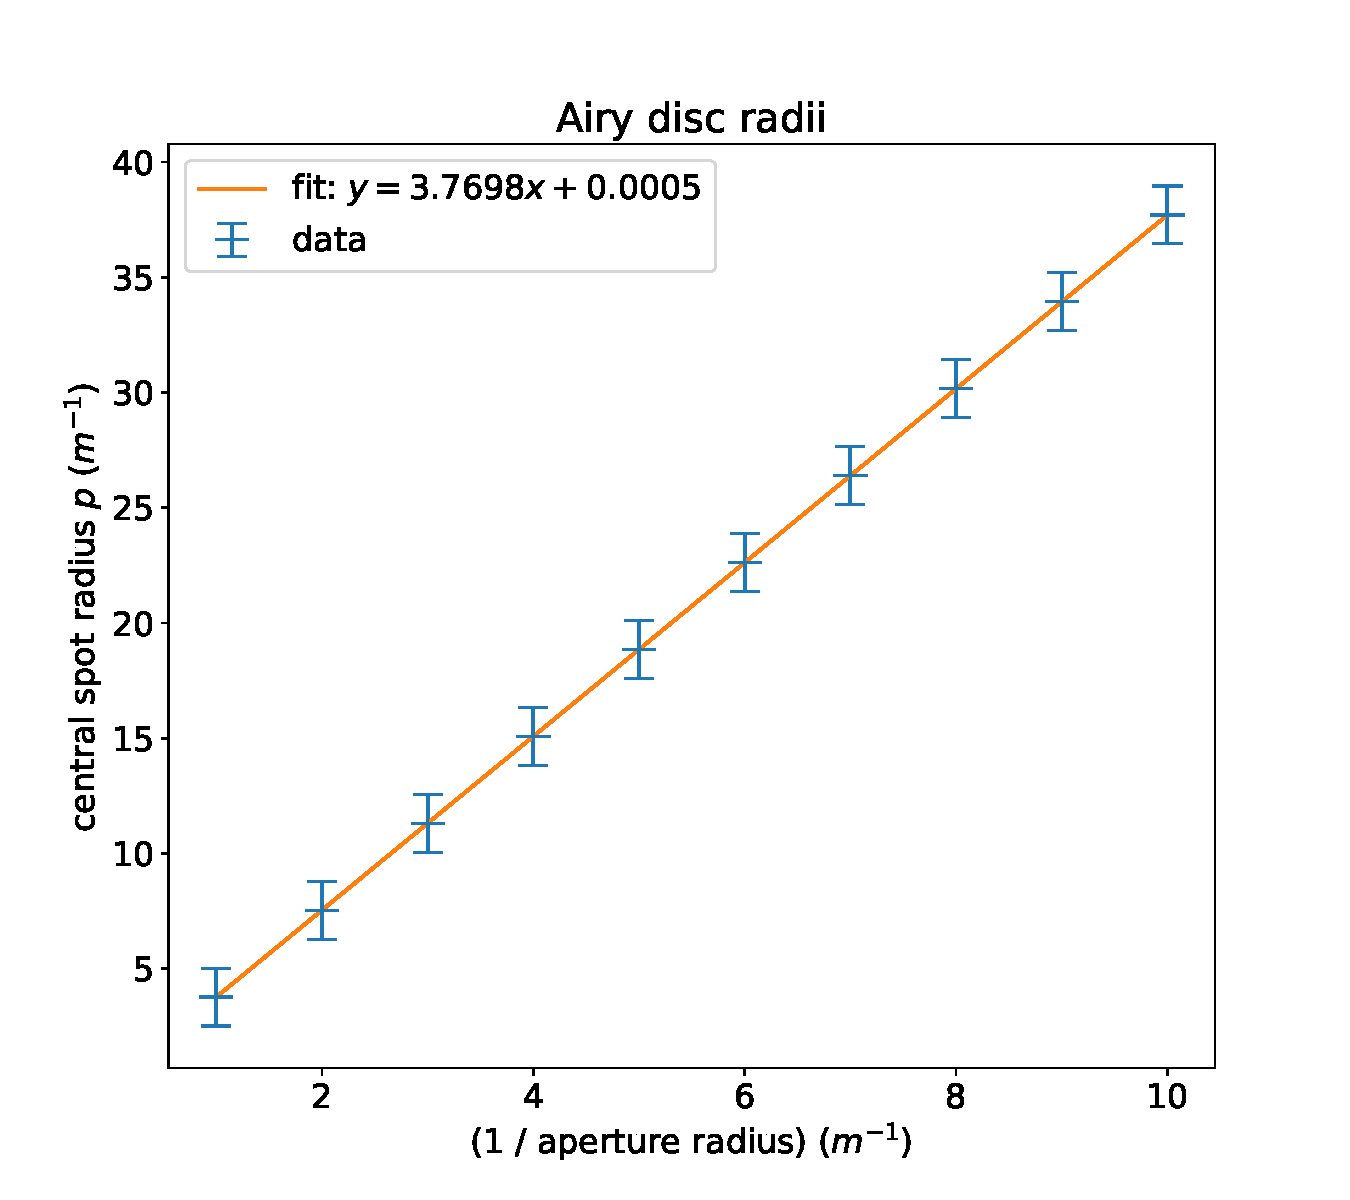
\includegraphics[width=\textwidth]{pictures/tests/airy.pdf}
        \caption{}\label{fig:test1:round}
    \end{subfigure}%
    \begin{subfigure}{0.5\textwidth}
        \centering
        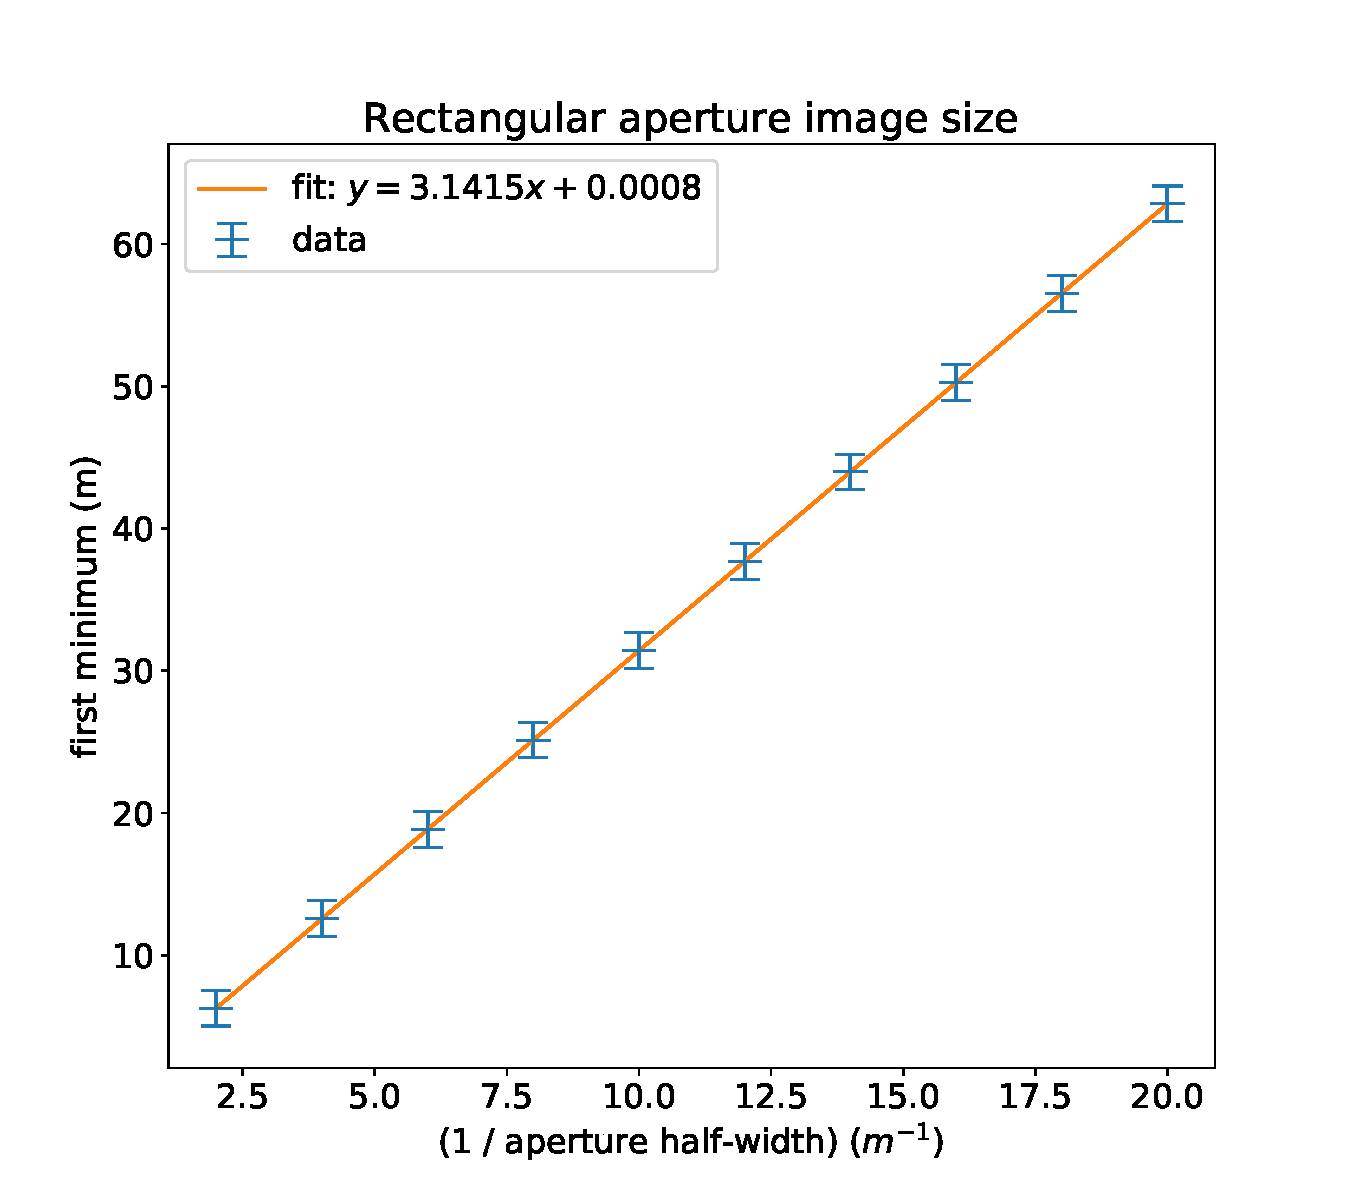
\includegraphics[width=\textwidth]{pictures/tests/rect.pdf}
        \caption{}\label{fig:test1:rect}
    \end{subfigure}
    \caption{Sizes of central spots as function of aperture size, for both round and rectangular apertures.}\label{fig:test1}
\end{figure}

\begin{figure}
    \centering
    \begin{subfigure}{0.5\textwidth}
        \centering
        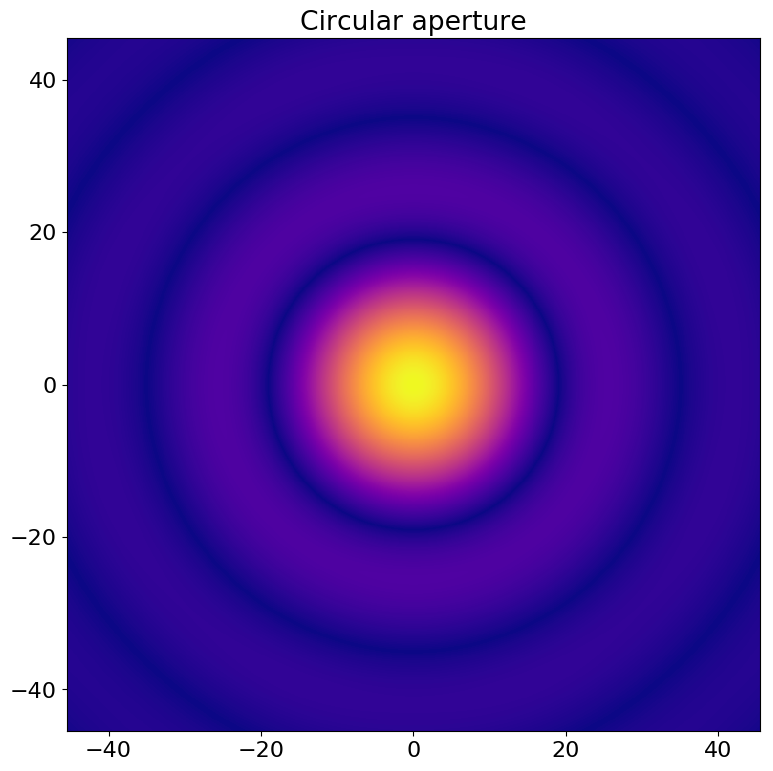
\includegraphics[width=\textwidth]{pictures/def/out0}
        \caption{}\label{fig:typ:round}
    \end{subfigure}%
    \begin{subfigure}{0.5\textwidth}
        \centering
        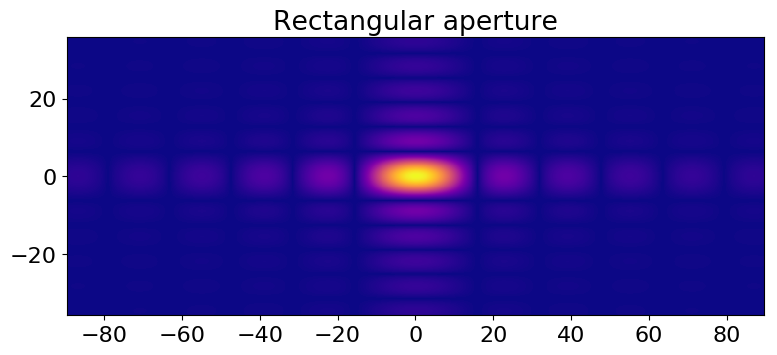
\includegraphics[width=\textwidth]{pictures/def/out1}
        \caption{}\label{fig:typ:rect}
    \end{subfigure}
    \caption{Typical diffraction patterns of circular and vertical rectangular apertures.}\label{fig:typ}
\end{figure}

First, I ran the program on series of circular and rectangular apertures described in \texttt{config/circular\_mins.txt} and \texttt{config/rectangle\_mins.txt}, expecting to see a linear relationship between the extent of the central maximum and the inverse of the aperture size (see Section~\ref{sec:analysis:test}). As seen in Figure~\ref{fig:test1}, these linear relationships hold. The line slopes are close to the expected values of $1.22\pi$ for the Airy disc and $\pi$ for rectangular shapes.

Figure~\ref{fig:typ} shows that the diffraction patterns look as expected. Most notably, the image from a vertical rectangle is longer along the horizontal axis, as expected from Equation~\ref{eqn:test_rect}.

\section{Conclusion}\label{sec:conclusion}

\printbibliography{}
\end{document}